\section{Nebenläufigkeit, Transaktionen}
\label{sec:parallel}

\textbf{Synchronisation}
\begin{items}
	\item Viele Nutzer sollen Daten gleichzeitig lesen und schreiben können
		\\*
		\( \leadsto \) Konsistenz sicherstellen \( \leadsto \) \textbf{Synchronisationskomponente}
	\item Nutzer soll denken, er wäre der einzige
	\item \underline{Serielle Ausführung}: 
		\\*
		+ Konsistenz immer gewährleistet 
		\\*
		- extreme Wartezeiten
	\item \underline{Nicht-serielle Ausführung}:
		\\*
		- Lost Updates
		\\*
		- inkonsistente Lesezugriffe
		\\*
		- Dirty Reads (Reads von nicht-übermittelten Updates)
		\\*
		- Phantome
\end{items}

\textbf{Lost Update}
\begin{items}
	\item Programm \( T_1 \) transferiert 300 EUR von Konto \( A \) nach Konto \( B \),
		\\*
		Programm \( T_2 \) schreibt Konto \( A \) \( 3 \% \) Zinsen gut
		\\*
		\( \leadsto \) Zinsen aus \( S_5 \) von \( T_2 \) verloren, weil \( T_1 \) in \( S_6 \) überschreibt
\end{items}
\begin{figure}[H]\centering\label{Synchronisation}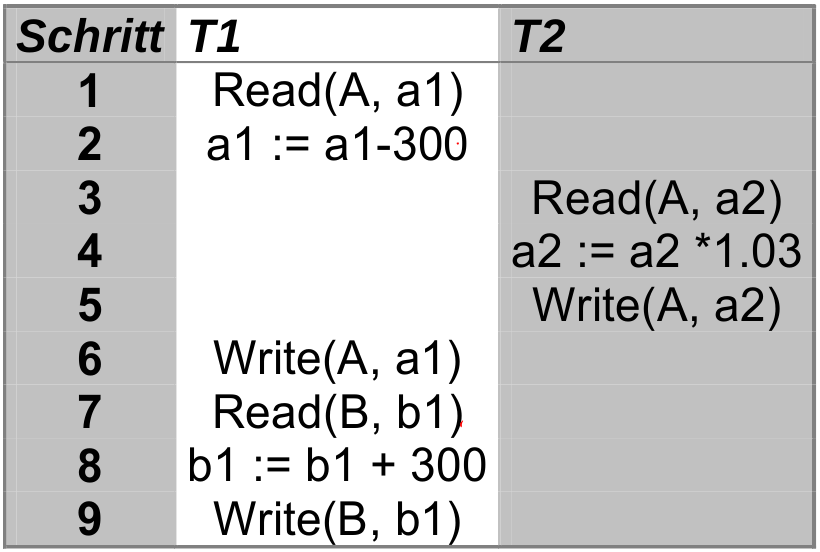
\includegraphics[width=0.2\textwidth]{Synchronisation}\end{figure}

\textbf{Dirty Read}
\begin{items}
	\item = Commit, Abort
	\item \( T_2 \) schreibt Zinsen git basierend auf einem Wert, der nicht zu einem konsistenten Zustand gehört, denn später erfolgt Abort von \( T_1 \)
\end{items}
\begin{figure}[H]\centering\label{DirtyRead}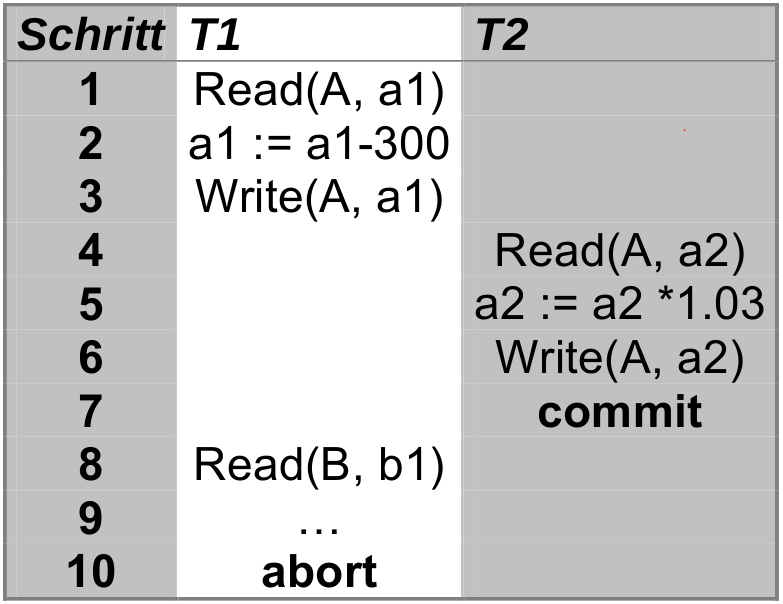
\includegraphics[width=0.2\textwidth]{DirtyRead}\end{figure}

\textbf{Non-Repeatable Reads}
\begin{items}
	\item Programm liest Datenobjekt mehr als einmal und sieht Änderung durch anderes Programm
\end{items}
\begin{figure}[H]\centering\label{NonRepeatableRead}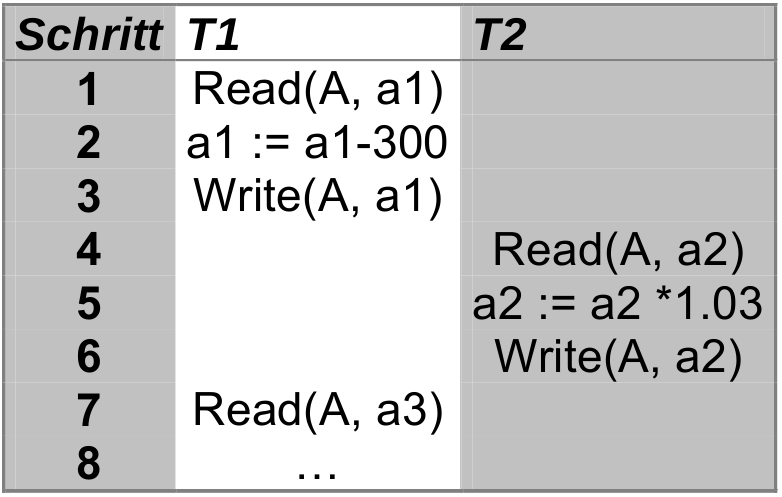
\includegraphics[width=0.2\textwidth]{NonRepeatableRead}\end{figure}

\textbf{Transaktionen}
\begin{items}
	\item = Ausführung eines Programms, dass auf DB (lesend oder schreibend) zugreift
	\item Zwei Operationen \( p, q \) konlfligieren
		\\*
		\( \Leftrightarrow \) \( p,q \) greifen auf selbes Datenobjekt zu und \( p \) oder \( q \) ist Schreiboperation
\end{items}

\textbf{Histories}
\begin{items}
	\item \underline{Vollständige Historie}: Menge von Transaktionen und Ausführungsordnung (nebenläufige Verzahnung)
	\item \underline{Historie}: Präfix einer vollständigen Historie
	\item \underline{Commited Projection} (\( C(H) \)): H nach Entfernen aller nicht-committeten Operationen
	\item Korrektheit im Fehlerfall:
	\begin{enumeration}
		\item \( \alpha \) = ``History enthält <10 Operationen'': 
			\\*
			Erfüllt \( H \) \( \alpha \), dann auch Präfixe \( H', H'', \dots \)
			\\*
			\( \leadsto \) \( \alpha \) ist \textbf{prefix commit-closed}
		\item \( \beta \) = ``Alle Operationen sind Leseoperationen'':
			\\*
			Erfüllt \( H \) \( \beta \), dann auch \( H', H'', \dots \)
			\\*
			\( \leadsto \) \( \beta \) ist prefix commit-closed
		\item \( \gamma \) = ``History enthält mehr als 10 Operationen'':
			\\*
			\( H' \) muss \( \gamma \) nicht erfüllen \\*
			\( \leadsto \) \( \gamma \) ist nicht prefix commit-closed
	\end{enumeration}
	\item Eine Eigenschaft von Histories ist prefix commit closed
		\\*
		\( \Leftrightarrow \) (\( H \) erfüllt Eigenschaft \( \Rightarrow C(H') \) erfüllt Eigenschaft)
\end{items}

\textbf{Konfliktäquivalenz}
\begin{items}
	\item \( H, H' \) (Konflikt-)Äquivalent, wenn
	\begin{enumeration}
		\item gleiche Transaktionen, gleiche Operationen
		\item gleiche Ordnung konfligierender Operationen
	\end{enumeration}
\end{items}

\textbf{Serialisierbarkeit}
\begin{items}
	\item \( H \) serialisierbar \( \Leftrightarrow C(H) \equiv H_S \) (serielle History)
	\item \underline{Serialisierbarkeitsgraph} (Abhängigkeitsgraph):
		\\*
		Knoten = Transaktionen
		\\*
		(gerichtete) Kante = Abhängigkeit zwischen Transaktionen: Transaktionen greifen auf selbes Datenobjekt zu \( \leadsto \) Operationen konfligieren
	\item Theorem: Schedule ist serialisierbar, wenn entsprechender Abhängigkeitsgraph zykelfrei ist
	\item \textbf{Ansatz nicht praktikabel}:
	\begin{enumeration}
		\item Serialisierbarkeit von Schedules nur im Nachhinein überprüfbar
		\item Administrativer Overhead zu hoch: Abhängigkeiten zu bereits terminierten Transaktionen berücksichtigen
	\end{enumeration}
\end{items}

\textbf{Locking}
\begin{items}
	\item Lock für jedes Datenobjekt und jede Operationsart
		\\*
		Notation: \( ol_i[x] \)
	\item Einfachster Fall: Nur Read/Write Locks
		\\*
		\( \leadsto \) \emph{rx locking scheme}
	\item \underline{Zwei-Phasen-Sperrprotokoll}:
	\begin{enumeration}
		\item Locks werden hinzugenommen
		\item Locks werden freigegeben
	\end{enumeration}
	\( \leadsto \) stellt Serialisierbarkeit sicher
\end{items}

\textbf{Deadlock}
\begin{items}
	\item \( T_1: r_1[x] \to w_1[y] \to c_1, T_2: w_2[y] \to w_2[x] \to c_2 \)
	\begin{enumeration}
		\item Beide Transaktionen zuerst keine Locks
		\item TM sendet \( r_1[x] \) an Scheduler
			\\*
			\( \leadsto rl_1[x] \), Scheduler sendet \( r_1[x] \) an DM
		\item TM sendet \( w_2[y] \) ab Scheduler
			\\*
			\( \leadsto wl_2[y] \), Scheduler sendet \( w_2[y] \) an DM
		\item TM sendet \( w_2[x] \) an Scheduler
			\\*
			\( \leadsto wl_2[x] \) nicht möglich \( \leadsto \) Verzögerung
		\item TM sendet \( w_1[y] \) an Scheduler
			\\*
			\( \leadsto wl_1[y] \) nicht möglich \( \leadsto \) Verzögerung
	\end{enumeration}
	\( \leadsto \) \textbf{Deadlock}
\end{items}

\textbf{Strenges 2-Phasen-Sperrprotokoll}
\begin{items}
	\item Freigabe der Locks erst nach Transaktionsende
\end{items}

\begin{fragen}
	\begin{enumeration}
		\item Was ist Isolation? Was ist der Zusammenhang zwischen Isolation und Serialisierbarkeit?
		\item Welche Probleme können bei unkontrollierter nebenläufiger Ausführung von Transaktionen auftreten?
		\item Beispiele für Lost Updates, Non-Repeatable Reads usw. angeben, die bestimmte Bedingungen erfüllen
		\item Warum ist es wichtig, dass unser Korrektheitskriterium für Histories prefix commit closed ist? Erklären Sie, warum Konflikt-Serialisierbarkeit prefix commit closed ist.
		\item Ist eine gegebene History serialisierbar/recoverable/cascadeless?
		\item Haben zwei Konflikt-äquivalente Histories stets die gleichen Reads-from-Beziehungen?
		\item Warum verwendet man in der Regel nicht den Serialisierbarkeitsgraphen, um Serialisierbarkeit sicherzustellen?
		\item Bei Deadlocks wird in der Regel eine Transaktion zurückgesetzt. Kann es vorkommen, dass die gleiche Transaktion mehrmals/beliebig oft zurückgesetzt wird? Wenn ja, was kann man jeweils dagegen tun?
		\item Geben Sie ein Beispiel für eine serialisierbare Ausführung, bestehend aus drei Transaktionen, mit folgender Eigenschaft an: Die zeitliche Reihenfolge der Commits ist \( c_1 \) vor \( c_2 \) vor \( c_3 \), die der äquivalenten seriellen Ausführung jedoch \( c_3 \) vor \( c_2 \) vor \( c_1 \).
		\item Um einen Deadlock aufzulösen muss eine der beteiligten Transaktionen zurückgesetzt werden. Welche Kriterien sind Ihres Erachtens nach sinnvoll, um diese Auswahl zu treffen?
	\end{enumeration}
\end{fragen}